\documentclass[12pt]{article}
\usepackage{listings}
\usepackage[colorlinks=true,pagebackref,linkcolor=blue]{hyperref}
\usepackage{graphicx}
\textwidth=7in
\textheight=9.5in
\topmargin=-1in
\headheight=0in
\headsep=.5in
\hoffset  -.85in


\lstset{
basicstyle=\footnotesize\ttfamily,
language=bash,
upquote=true,
breakatwhitespace=true,
columns=fullflexible,
keepspaces,
%numbers=none,
tabsize=3,
frame=blrt,
framextopmargin=5pt,
showstringspaces=false,
extendedchars=true
}

\pagestyle{empty}

\renewcommand{\thefootnote}{\fnsymbol{footnote}}

\begin{document}



\begin{center}
{\bf AMS 550.400 \quad HW SET 1\quad  Due Date:  Oct 10}\\

{\bf Yen Theng Tan}\\
\vskip.2in
{\footnotesize Last Compiled on \today}
\end{center}

\setlength{\unitlength}{1in}

\begin{picture}(6,.1) 
\put(0,0) {\line(1,0){6.25}}         
\end{picture}

 

\renewcommand{\arraystretch}{2}


\vskip.25in
\noindent\textbf{Problem 1 (10 pts):}  
\vskip.25in


mkdir qn1.git % makes directory

cd qn1.git

git init .

vi main.txt % Add A

git add .

git commit -m "A added"

vi main.txt %Add B 

git add .

git commit -m "B added"

git branch alt % creates alt branch with commits A and B

vi main.txt

git add .

git commit -m "C added"% commit C at master branch, alt branch not affected

git checkout alt% moves to alt branch

vi main.txt % add X

git add .

git commit -m "X added"

git checkout master

git merge alt %merges and resolves conflicts

vi main.txt

git add .

git commit -m "merged"

vi main.txt

git add .

git commit -m "D added"

git log --graph --oneline

git checkout alt

git log --graph --oneline


\newpage

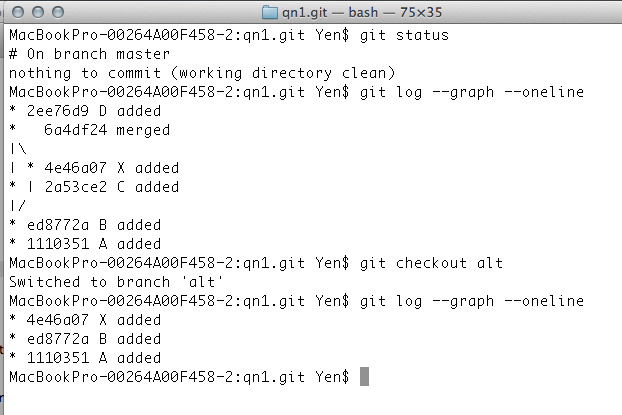
\includegraphics[width=\textwidth]{graph.png}

%PROBLEM 2
\newpage
\vskip1in
\noindent\textbf{Problem 2 (10 pts):}
\vskip.25in

git config --global user.name "Yen Theng Tan"

git config --global user.email yen@jhu.edu

git remote add s1 git://github.com/nhlee/550400.stanza1.git

git remote add s2 git://github.com/nhlee/550400.stanza2.git

git remote add s3 git://github.com/nhlee/550400.stanza3.git

mkdir poem.git

cd poem.git

git init .

git pull s1 master

vi main.txt % add title

git pull s2 master

git pull s3 master

vi main.txt % merge conflict

git add .

git commit -m "merged"

git remote add myrepo https://github.com/yenz88/550400.homeworkset.1

git push myrepo master %push to newly created repository



\newpage
\noindent\textbf{Problem 3 (40 pts):}
\vskip.25in

Team projects require collaboration among its members. This process can potentially be time-consuming, and an inefficient method of collaboration can even have a negative effect on the outcome of the project. We are considering a team of 4 students (“A”, “B”, “C”, and “D”) who are working on writing a latex/beamer file (“main.tex”) for a class presentation of their work statement. Specifically, A is in charge of the Introduction/Preamble, B is in charge of the Problem Statement, C is in charge of the Timeline, and D is in charge of the Deliverables. They do not wish to coordinate their schedules for a concurrent group meeting, either online or in person. In terms of their work allocations, their contributions to main.tex do not overlap. We want to devise two work flow strategies for the team so that they can collaborate asynchronously using git. We will then compare the two strategies and make a final recommendation. 

The exogenous variables are the four contributions from the four respective members of the team, as they are the parameters for the work flow strategies. These exogenous variables combine to form the final product, which is the merged main.tex file, and this is the endogenous variable. The work flow strategy that we are recommending (i.e. the method using which the four members will collaborate) is the function. Unimportant variables include the length of each contribution and the sequence in which the contributions are compiled.

The first strategy is to create a central git repository, and have all four members create their own respective git repositories. The members would work on their respective pieces separately and push their work to their own repositories. When ready to combine their work, the lead member of the team will then pull all the submissions from the four git directories, and merge all their ‘conflicts’, which is presumably none because they are working on separate parts of the project. However, he will have to ensure that the four contributions are merged correctly into the central repository. 

The second strategy is to create a single central git repository, and create four branches, one for each member. Whenever they work on the project, they will have to work from their respective branches. Once done, from the master branch, they can merge all the respective branches, remove any conflicts, and assemble their project. 

Both strategies allow the team members to work independently of each other, and not work on the same folder in the same branch. However, the first strategy separates the work using different repositories, and this allows different members to keep track of their own work in a clearer and more distinct manner. They can push and pull to their own repository without affecting anyone else, and they will have a separate copy on their own. The second strategy utilizes git more by creating separate branches. Once more, they can work on their own submissions on these respective branches, but on a common repository. This makes it easier to keep track of all the member’s work, but it also carries some risks because data can be accidentally merged or deleted, and the whole project is reliant on one repository. 

The first strategy, while providing greater security and separation among the members, also makes it more difficult to see what others are doing. Since the contributions of this particular project do not overlap, and they can work independently of each other, but it is often useful to keep track of their work. To do this, members must pull from each other’s repositories in order to view it. However in the second strategy, this can be done much quicker by switching branches and viewing their work. Also, should there be a common change that all team members must view and make from the master file, in the first strategy this can be achieved by merging from their own respective branches. Thus, given the ease of viewing and merging their files, and assuming that project security is not a top priority, we would suggest using the second strategy – creating a central repository and four branches, one for each team member. 



\newpage
\noindent\textbf{Problem 4 (aka.\ Fair Play, 40 pts):}
\vskip.25in

We want to find out if tennis is fair, with regard to the structure of the game. Assuming that both players are equal in skill, in both serving and returning a serve, is this sport fair to both players? We also assume that the server always has an advantage, since he or she has the time and initiative of firing the ball first, and the other player has to react to this, usually resulting in a weaker return compared to the serve. Given this advantage in serving, is the tennis still fair to both players? 

First we must determine in what manner the serve affects the match as a whole. A tennis match is composed of points, games and sets. Assuming a best of 5 format, a player has to win 3 sets to win the match. To win a set, a player has to be the first to win at least 6 games and by at least 2 games. If both players have won 6 games each in a single set, they head for a tiebreak where the player wins the set by scoring at least 7 points and winning by at least 2 points in this tiebreak game. The player who is supposed to serve in the next game serves in this tiebreak game. In a normal non-tiebreak game, players win the game by scoring at least 4 points and by at least 2 points. Given this information, the exogenous variables are the points, games, sets and to whom the service is awarded to in each of these, whether it is player A or player B.  The endogenous variable will be the winner of the match, given whether player A or player B serves. 

For simplicity, since we assume that both players are equal in skill and that serving is advantageous, we shall also assume that the player who serves the game will win the game (only one player serves during the entire game, and thus he has the advantage throughout the game). Under this assumption, we consider the first set where player A serves first, and conclude that he will win the first game, and player B (who serves next) will tie the number of games, and so on and so forth. Thus, each set will always result in a tiebreak. Analyzing the tiebreak, we see that Player A serves first in the tiebreak and wins the first point (1-0). (In a tiebreak, the next designated server serves the first point, and subsequently players serve two consecutive points each before handing over the serve). Player B then wins the next two points (1-2), and the serve returns to player A, who wins the next two points (3-2), and so on. Here we see that there is no decided winner even if we restrain the model to assume that the server wins the point.  Thus, if there is no causal relationship between a player’s performance and the previous point he played, we see that the tiebreak point structure in each set prevents any unfair advantage of service. 

In reality, there does exist a correlation between a player’s performance and the result of the previous point/game/set being played. However, this correlation is highly qualitative, and it is questionable whether it can be quantitatively modeled. For example, a player who lost the previous point/game/set may be discouraged and perform worse, or he might be spurred on and perform better. To see how this can affect our model, and in fact provide us with a conclusive result, we assume that winning a point/game gives momentum and increases the probability of winning. We also assume that each set is independent of each other. Applying this back to our previous example, player A who serves first will win the tiebreak, and the first set. Player B will win the second set by the same logic, tying the sets at 1-1. Since the player who wins 3 sets first wins the match, player A will win if he serves first. If the entire universe of tennis players behaves this way, then the sport of tennis will be considered unfair, because service will likely determine the winner. 

Thus, this model is useful only if we can accurately quantify the behavior and performance of all players after they have won or lost the previous point/game/set, since these assumptions will give tell us whether the structure of tennis is fair or not. Since it is surely that each player behaves differently post-point, and assuming that half of time they perform better and half of the time they perform worse, the tiebreak structure rewards the better tennis player, regardless of his serve, and thus the sport of tennis can be considered fair. 

\end{document}
